% Chapter 5

\chapter{Implementation and Results} % Write in your own chapter title
\label{Chapter5}
\lhead{Chapter 5. \emph{Implementation \& Results}} 
\section{System Requirements}
\lstdefinestyle{python}{
    language=Python,
    basicstyle=\ttfamily\footnotesize, % Use a monospaced font and smaller size
    keywordstyle=\bfseries\color{blue},
    stringstyle=\color{green},
    commentstyle=\color{gray},
    numbers=left, % Line numbers on the left
    numberstyle=\tiny\color{gray},
    stepnumber=1,
    numbersep=10pt,
    frame=single, % Frame around the code block
    breaklines=true, % Enable line breaking
    breakatwhitespace=true, % Only break at whitespace
    tabsize=4, % Set tab size to 4 spaces
    showspaces=false, % Do not display spaces
    showstringspaces=false, % Do not display spaces in strings
    showtabs=false, % Do not display tabs
}
\subsection{Hardware requirements}
As the final product is a software suite, different systems and environments are required to run and coexist. The desktop application requires a minimum of core i5 10th gen processor with 8 GB RAM and 128 GB SSD. Developed in PyQt5, it can be run on Linux, Mac, and Windows OS. The IP cameras used are two mega-pixels (MP) that require network configuration and a readily available internet connection with high bandwidth to send IoT messages and surveillance video to the desktop. The portal is web-based, so it requires no specific operating system to run be it Windows, Linux, or Mac OS. The portal will require a RAM of 8 GB and a processor with specifications i5 8th generation or above. The web server deployed on the cloud service requires a high power multiprocessor to process a large number of requests at a time; thus the distributed computing infrastructure offered by the AWS CloudFormation service is preferable.

\subsection{Software requirements}
The software utilizes multiple third party storage services namely:
\begin{itemize}
    \item \textbf{MMAction2:} Framework used to integrate pre-trained temporal activity localization and recognition models.
    \item \textbf{YoloV5:} Object detection model for tagging and tracking patients.
    \item \textbf{Google-API:} API client used to authenticate the user email address.
    \item \textbf{InfluxDB Cloud 2.0:} Store the patient activity logs.
    \item \textbf{Azure Storage:} Store images and clips of patient when an emergency is detected by the system.
    \item \textbf{PostGreSQL:} Store the user information and the rest of the system database.
\end{itemize}
The system also utilizes \textbf{Stripe's} payment gateway to facilitate online payments. The application backend developed in Python's Django framework was deployed on \textbf{Vercel}.
To communicate IoT messages to the Django web app, a high-bandwidth communication third-party service is integrated, namely, \textbf{Pusher} and \textbf{HiveMqtt}, which are essentially web sockets in nature. They utilize Mqtt and web socket communication protocols for communication. To facilitate the upload and download of pdf files, \textbf{FTP} is used, and \textbf{HTTP} has been used to facilitate client-server communications. Firebase cloud messaging is used to provide push notifications. To allow users to use two-factor authentication (2FA), \textbf{SMTP and POP3} are used to send an email, and \textbf{SMPP} is used for sending an SMS containing a one-time password (OTP). 
\subsection{Deployment}
Developing the desktop app in the PyQt5 framework allows the application to run cross-platform. Using Pyinstaller the application is converted into a single .exe application allowing easy installation. The backend developed in Django is deployed on Vercel in the free tier version. Frontend is deployed on Netlify and cross-origin scripting is ensured with Netlify app as the only allowed origin. The system was tested in a controlled environment within the research lab by integrating an IP Camera of 2 MP and using the project members as test subjects for activity recognition and logging.
\subsection{Training \& Testing of BSN}
\subsection{Dataset}
We used two main datasets for our study: ActivityNet-1.3 and THUMOS14. ActivityNet-1.3 consists of 19,994 videos with 200 action classes. It was used in the ActivityNet Challenges in 2016 and 2017. The dataset was divided into training, validation, and testing sets in a 2:1:1 ratio. THUMOS14 contains 200 and 213 temporally annotated untrimmed videos with 20 action classes in the separate validation and testing sets, respectively. The training set of THUMOS14 was sourced from UCF-101, which contains trimmed videos for action recognition.

\subsection{Training}
We used a two-stream network architecture for visual feature encoding, with BN-Inception serving as the temporal network and ResNet as the spatial network. This architecture was implemented using Caffe and pre-trained on the training set of ActivityNet-1.3. During feature extraction, we set the interval of the snippets to 16 on ActivityNet-1.3 and 5 on THUMOS14.

On ActivityNet-1.3, to account for the limited duration of the videos, we rescaled the feature sequence of each video to a new length of 100 using linear interpolation. The corresponding annotations were  adjusted to fit within the range [0,1]. The temporal and proposal evaluation modules in BSN were implemented using TensorFlow. We trained the temporal evaluation module with a batch size of 16 and  learning rate of 0.001 for 10 epochs, followed by 0.0001 for 10 epochs. The proposed evaluation module was trained using a batch size of 256 and the same learning rate.
\subsubsection{Temporal Evaluation Module}
The temporal evaluation module is designed to assess the probabilities of event start, end, and actionness across all temporal locations within a video. It employs three temporal convolutional layers to extract temporal features, utilizing Rectified Linear Unit (ReLU) activation functions for the first two layers and a Sigmoid activation function for the last layer to generate probability values.
    \begin{lstlisting}[style=python]
    class TEM(torch.nn.Module):
    def __init__(self, opt):
        super(TEM, self).__init__()
        self.feat_dim = opt["tem_feat_dim"]
        self.temporal_dim = opt["temporal_scale"]
        self.batch_size= opt["tem_batch_size"]
        self.c_hidden = opt["tem_hidden_dim"]
        self.tem_best_loss = 10000000
        self.output_dim = 3  
        
        self.conv1 = torch.nn.Conv1d(
        in_channels=self.feat_dim,
        out_channels=self.c_hidden,
        kernel_size=3,
        stride=1,
        padding=1,
        groups=1
        )
        
        self.conv2 = torch.nn.Conv1d(
        in_channels=self.c_hidden,
        out_channels=self.c_hidden,
        kernel_size=3,
        stride=1,
        padding=1,
        groups=1
        )
    
        self.conv3 = torch.nn.Conv1d(
        in_channels=self.c_hidden,
        out_channels=self.output_dim,
        kernel_size=1,stride=1,
        padding=0
        )
        self.reset_params()
        

    @staticmethod
    def weight_init(m):
        if isinstance(m, nn.Conv2d):
            init.xavier_normal(m.weight)
            init.constant(m.bias, 0)

    def reset_params(self):
        for i, m in enumerate(self.modules()):
            self.weight_init(m)

    def forward(self, x):
        x = F.relu(self.conv1(x))
        x = F.relu(self.conv2(x))
        x = torch.sigmoid(0.01*self.conv3(x))
        return x
    \end{lstlisting}

    \subsubsection{Proposed Generation Module}
    
The proposed generation module aims to identify and create proposals for significant regions of interest within a video. It follows a two-step process: first, identifying time intervals with very high boundary probabilities to define starting and ending points; second, combining these intervals to form complete proposals. Each proposal is represented by a Boundary-Sensitive Proposal (BSP) feature, combining actionness sequences from starting, center, and ending regions. Finally, each proposal is represented by its starting and ending points along with its BSP feature.
\begin{lstlisting}[style=python]

def generateProposals(opt,video_list,video_dict):
    tscale = opt["temporal_scale"]    
    tgap = 1./tscale
    peak_thres= opt["pgm_threshold"]

    for video_name in video_list:
        tdf=pandas.read_csv("./output/TEM_results/"+video_name+".csv")
        start_scores=tdf.start.values[:]
        end_scores=tdf.end.values[:]        
        max_start = max(start_scores)
        max_end = max(end_scores)
        
        start_bins=numpy.zeros(len(start_scores))
        start_bins[[0,-1]]=1
        for idx in range(1,tscale-1):
            if start_scores[idx]>start_scores[idx+1] 
            and
            start_scores[idx]>start_scores[idx-1]:
                start_bins[idx]=1
            elif start_scores[idx]>(peak_thres*max_start):
                start_bins[idx]=1
                    
        end_bins=numpy.zeros(len(end_scores))
        end_bins[[0,-1]]=1
        for idx in range(1,tscale-1):
            if end_scores[idx]>end_scores[idx+1] 
            and
            end_scores[idx]>end_scores[idx-1]:
                end_bins[idx]=1
            elif end_scores[idx]>(peak_thres*max_end):
                end_bins[idx]=1
        
        xmin_list=[]
        xmin_score_list=[]
        xmax_list=[]
        xmax_score_list=[]
        for j in range(tscale):
            if start_bins[j]==1:
                xmin_list.append(tgap/2+tgap*j)
                xmin_score_list.append(start_scores[j])
            if end_bins[j]==1:
                xmax_list.append(tgap/2+tgap*j)
                xmax_score_list.append(end_scores[j])
                
        new_props=[]
        for ii in range(len(xmax_list)):
            tmp_xmax=xmax_list[ii]
            tmp_xmax_score=xmax_score_list[ii]
            
            for ij in range(len(xmin_list)):
                tmp_xmin=xmin_list[ij]
                tmp_xmin_score=xmin_score_list[ij]
                if tmp_xmin>=tmp_xmax:
                    break
                new_props.append(
                [
                tmp_xmin,tmp_xmax,
                tmp_xmin_score,
                tmp_xmax_score
                ]
                )
        new_props=numpy.stack(new_props)
        col_name=["xmin","xmax","xmin_score","xmax_score"]
        new_df=pandas.DataFrame(new_props,columns=col_name)  
        new_df["score"]=new_df.xmin_score*new_df.xmax_score
        new_df=new_df.sort_values(by="score",ascending=False)
        
        video_info=video_dict[video_name]
        video_frame=video_info['duration_frame']
        video_second=video_info['duration_second']
        feature_frame=video_info['feature_frame']
        corrected_second=float(feature_frame)/video_frame*video_second
        
        try:
            gt_xmins=[]
            gt_xmaxs=[]
            for idx in range(len(video_info["annotations"])):
                gt_xmins.append(
                video_info["annotations"][idx]["segment"][0]
                /
                corrected_second
                )
                gt_xmaxs.append(
                video_info["annotations"][idx]["segment"][1]
                /
                corrected_second
                )
            new_iou_list=[]
            for j in range(len(new_df)):
                tmp_new_iou=max(
                iou_with_anchors(
                new_df.xmin.values[j],
                new_df.xmax.values[j],
                gt_xmins,
                gt_xmaxs)
                )
                new_iou_list.append(tmp_new_iou)
                
            new_ioa_list=[]
            for j in range(len(new_df)):
                tmp_new_ioa=max(
                ioa_with_anchors(
                new_df.xmin.values[j]
                ,new_df.xmax.values[j],
                gt_xmins,gt_xmaxs)
                )
                new_ioa_list.append(tmp_new_ioa)
            new_df["match_iou"]=new_iou_list
            new_df["match_ioa"]=new_ioa_list
        except:
            pass
        new_df.to_csv("./output/PGM_proposals/"+video_name+".csv",index=False)
    \end{lstlisting}
\subsubsection{Proposal evaluation module}
    
The proposed evaluation module assigns confidence scores to each proposal, determining the likelihood of action occurrence within its duration. It employs a simple multilayer model with a hidden layer of 512 units using Rectified Linear Unit (ReLU) activation, and a sigmoid activation for the output layer to generate the confidence score. Each proposal is represented by its start and end time locations, along with starting and ending probabilities, and the confidence score.

\begin{lstlisting}[style=python]
class PEM(torch.nn.Module):
    
    def __init__(self,opt):
        super(PEM, self).__init__()
        self.feat_dim = opt["pem_feat_dim"]
        self.batch_size = opt["pem_batch_size"]
        self.hidden_dim = opt["pem_hidden_dim"]
        self.u_ratio_m = opt["pem_u_ratio_m"]
        self.u_ratio_l = opt["pem_u_ratio_l"]
        self.output_dim = 1
        self.pem_best_loss = 1000000
        
        self.fc1 = torch.nn.Linear(
        in_features=self.feat_dim,
        out_features=self.hidden_dim,
        bias =True
        )
        
        self.fc2 = torch.nn.Linear(
        in_features=self.hidden_dim,
        out_features=self.output_dim,
        bias =True
        )
        self.reset_params()

    @staticmethod
    def weight_init(m):
        if isinstance(m, nn.Conv2d):
            init.xavier_uniform_(m.weight)
            #init.xavier_normal(m.weight)
            init.constant(m.bias, 0)

    def reset_params(self):
        for i, m in enumerate(self.modules()):
            self.weight_init(m)

    def forward(self, x):
        x = F.relu(0.1*self.fc1(x))
        x = torch.sigmoid(0.1*self.fc2(x))
        return x
    \end{lstlisting}
\subsection{Result}
A crucial aspect of proposal generation methods is their ability to generate proposals for unseen action classes. To assess this, we selected two distinct action subsets from ActivityNet-1.3: "Sports, Exercise, and Recreation" and "Socializing, Relaxing, and Leisure" as seen and unseen subsets, respectively. The seen subset comprised 87 action classes with 4455 training and 2198 validation videos, while the unseen subset consisted of 38 action classes with 1903 training and 896 validation videos. The result were as follows:

\begin{figure}[H]
    \centering
    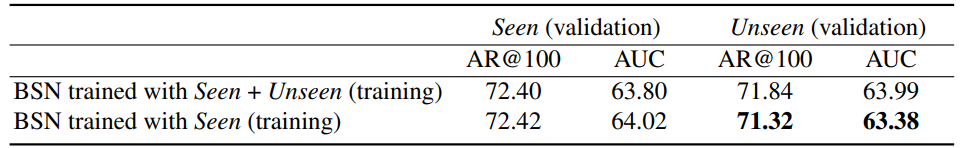
\includegraphics[width=\linewidth]{images/traing.png}
    \caption{Generalization Evaluation of BSN on ActivityNet-1.3. Seen Subset: “Sports, Exercise, and Recreation”; Unseen Subset: “Socializing, Relaxing, and Leisure”}
    \label{fig:BSN Evaluation}
\end{figure}
In our evaluation on the ActivityNet proposal task, our model achieved promising results. The Area Under the AR vs AN curve reached 67.42\%. For individual performance metrics, the model achieved an AR@1 of 32.93\%, AR@5 of 47.72\%, AR@10 of 55.59\%, and AR@100 of 75.12\%. These results indicate the effectiveness of the model in generating proposals for action recognition tasks.

\begin{figure}[H]
    \centering
    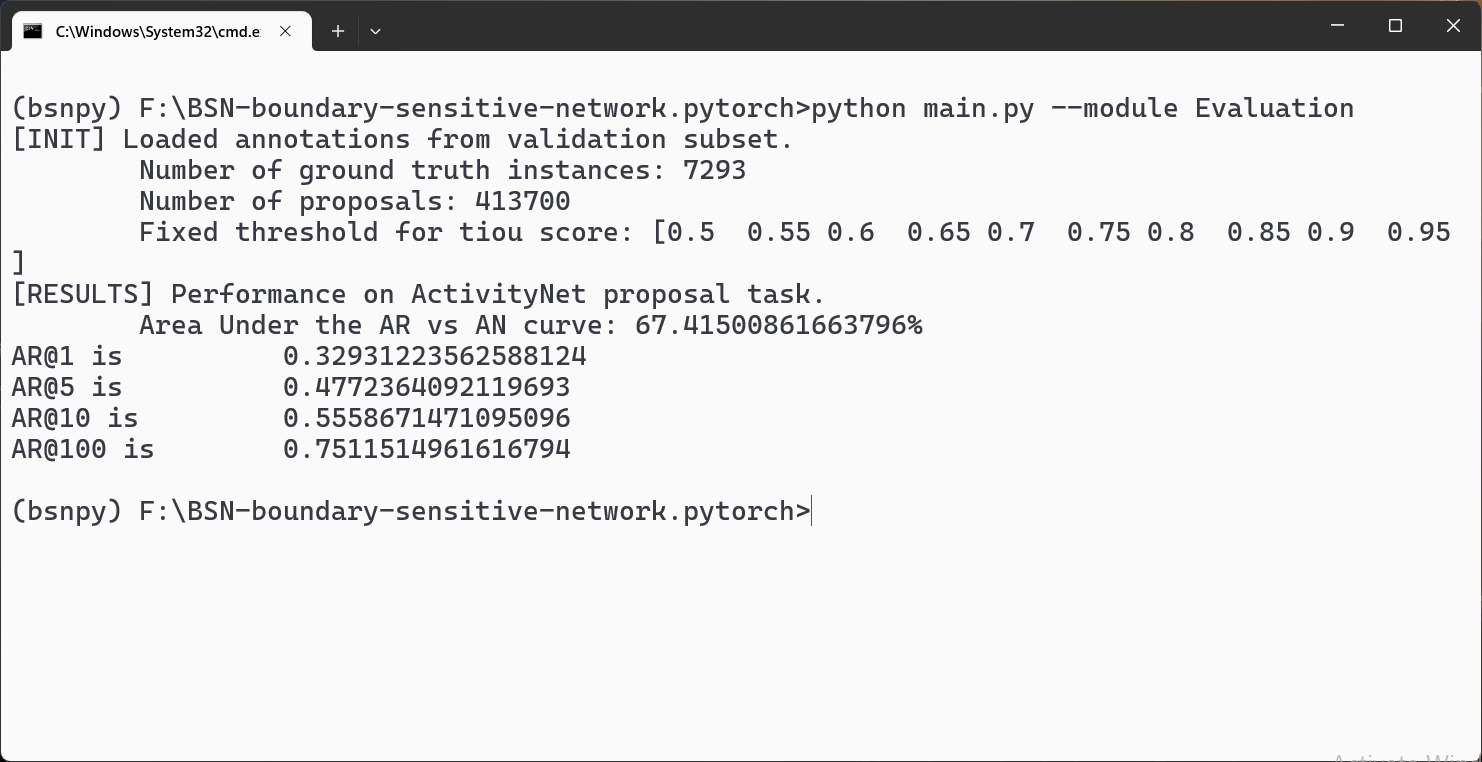
\includegraphics[width=0.8\linewidth]{images/result1.png}
    \caption{Model Accuracy}
    \label{fig:result CMD}
\end{figure}
\begin{figure}[H]
    \centering
    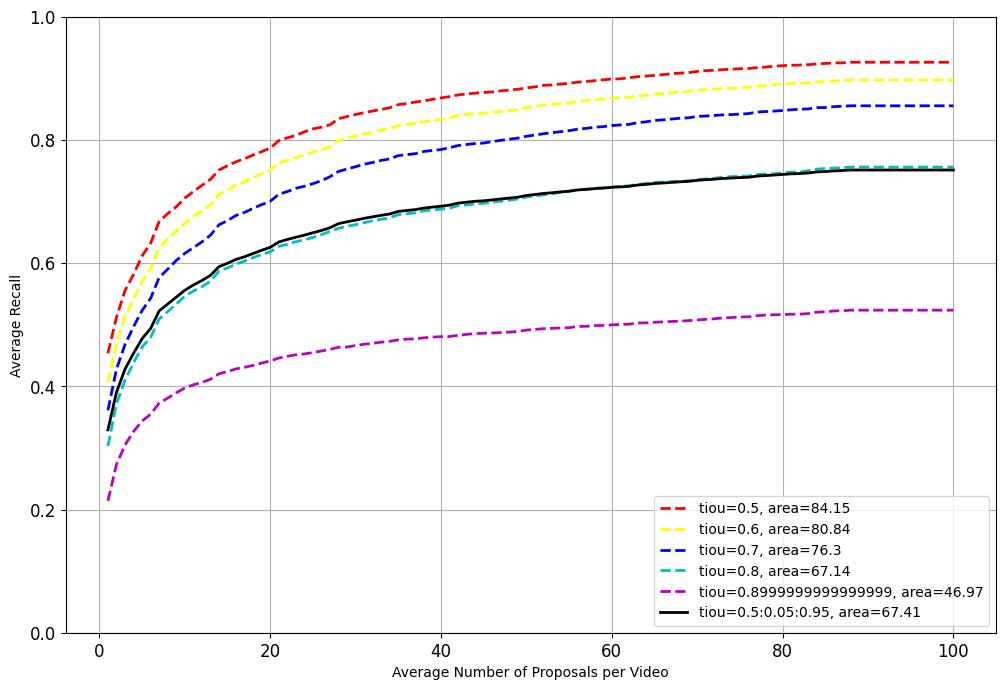
\includegraphics[width=0.7\linewidth]{images/result2.jpg}
    \caption{Relationship Between Average Recall and Proposal per Video}
    \label{fig:BSN Results}
\end{figure}

\subsection{Implementation \& Results of Transformer}
\subsubsection{Dataset}
To train the TST Plus model we use the Balanced Toyota Smarthome Untrimmed (TSU) dataset with 31 activities. To get the annotated data set we use the Balanced Toyota Smarthome repository \cite{btsu}. We save the annotated data in a separate file. The file is such that it contains 351 training data and 185 validation data. Each item of the annotated training and validation data consists of the video name, one hot encoding, number of frames, and the duration of the activity. The following code outputs the data shape and format that is loaded into the google colab notebook as shown in figure  \ref{fig:training-data tst}.
\begin{lstlisting} [style=python]
train_data = content['train']
validation_data = content['val']
combined_data = []
for value in train_data:
  print("Video Name: ",value[0],"--One Hot: ",value[1].shape,"--Frames: ",value[2],"--seconds: ",value[1].shape[0],value[2]//16)
  for val in value[1]:
    combined_data.append(val)
np_combined = np.array(combined_data)
np_combined.shape
\end{lstlisting}
\begin{figure}[h]
    \centering
    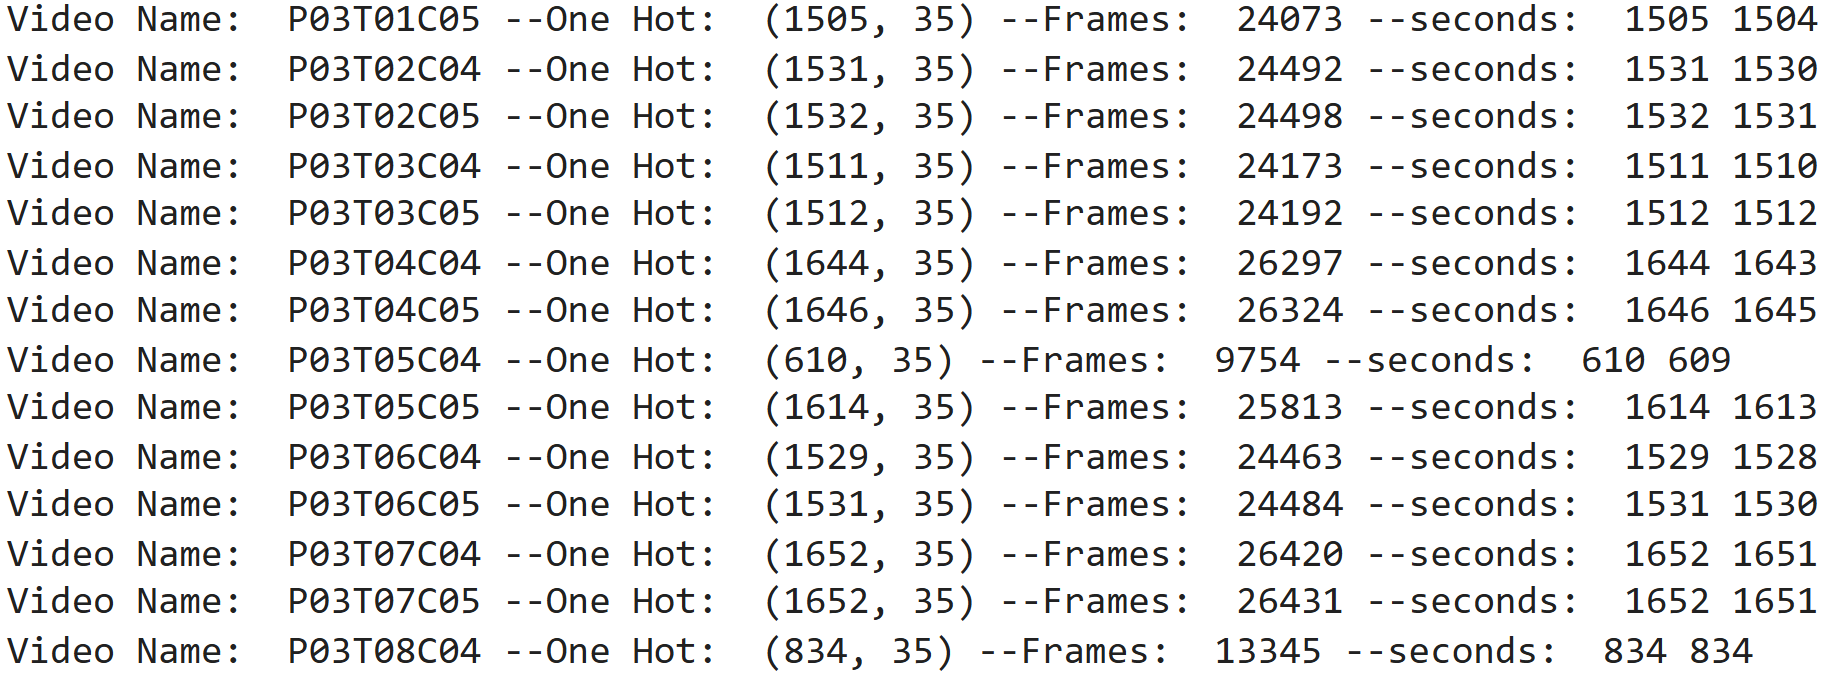
\includegraphics[width=0.7\linewidth]{images/trainingDataTST.png}
    \caption{Annotated Data}
    \label{fig:training-data tst}
\end{figure}

The training and validation data is further passed to the TST Plus model. We set the hyper parameters and number of iterations for training. The hyperparameters used in the training are:
\begin{enumerate}
    \item Learning rate: 1e-3
    \item Sliding window size: 32
    \item Horizon: 5
\end{enumerate}
\subsubsection{Model Training}
We use the TSAI \cite{tsai} library to forecast the activities of the patients. TSAI comprises of many forecasting models but we use the TST Plus to forecast the activities. The code for the TST Plus model's training is as shown below. Utilizing the pre-existing library provided by TSAI, the model is trained. Our input is the tuning of the hyper-parameters to give the most optimal forecasting accuracy
\begin{lstlisting}[style=python] 
from sklearn.metrics import accuracy_score , mean_squared_error , confusion_matrix
def activity_forecasting_model_training(forecasting_data , model, learning_rate , sliding_window_size , horizon , validation_size ,number_of_iterations):
  X, y = SlidingWindow(sliding_window_size, horizon=horizon)(forecasting_data)

  splits = TimeSplitter(validation_size, fcst_horizon=horizon)(y)

  tfms = [None, TSForecasting()]
  batch_tfms = TSStandardize()
  fcst = TSForecaster(X, y, path='models', splits = splits,tfms=tfms, batch_tfms=batch_tfms, bs=512, arch=model, metrics=mae )
  fcst.fit_one_cycle(number_of_iterations, learning_rate)

  raw_preds, target, preds = fcst.get_X_preds(X[splits[1]], y[splits[1]])
  return preds , target , raw_preds
\end{lstlisting}
The Model training output is shown in figures \ref{fig:training-split} and \ref{fig:training-model}. 
\begin{figure}[H]
    \centering
    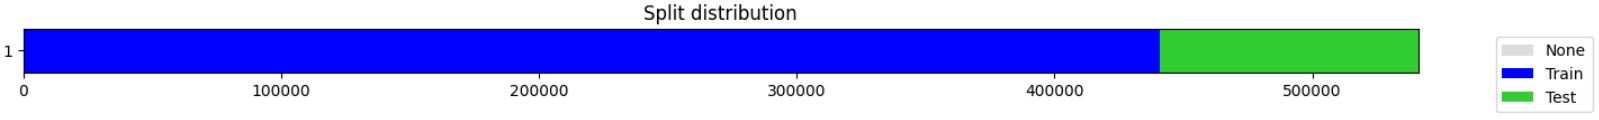
\includegraphics[width=\linewidth]{images/training split.png}
    \caption{Training Split for TST Plus Model}
    \label{fig:training-split}
\end{figure}
\begin{figure}[H]
    \centering
    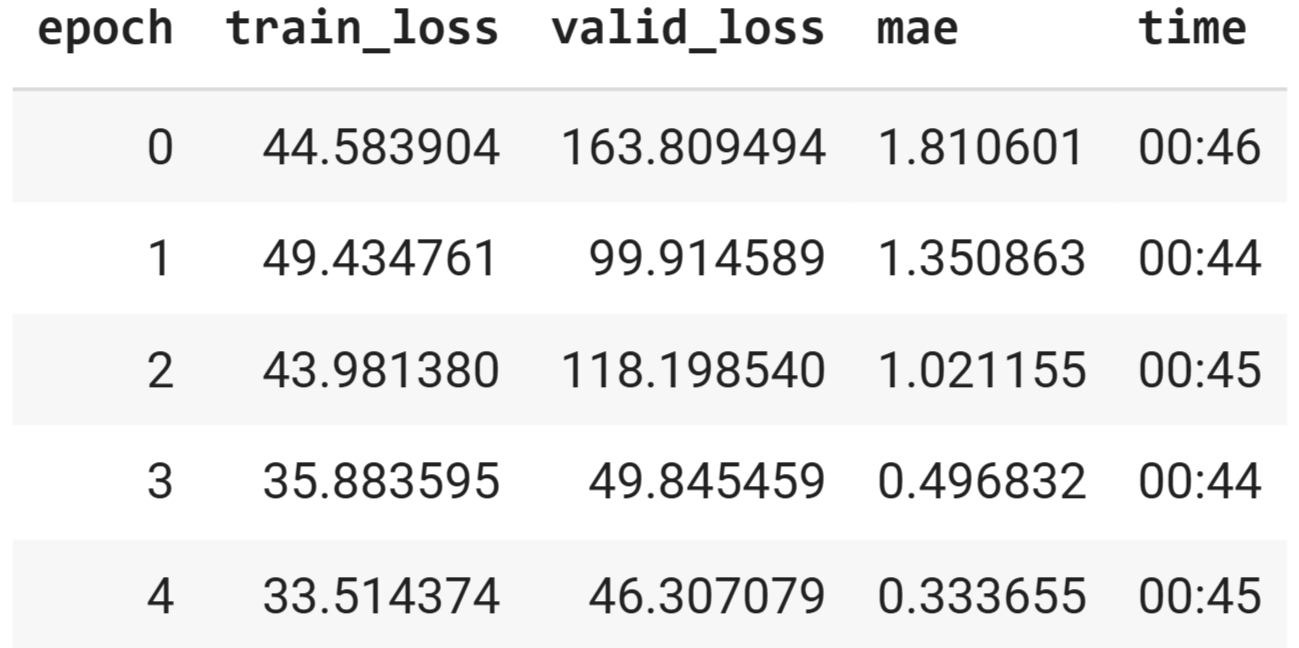
\includegraphics[width=0.7\linewidth]{images/training model.png}
    \caption{Training Results}
    \label{fig:training-model}
\end{figure}



\subsubsection{Results}
Due to limited resources we were not able to fully explore the potential of the TST forecaster as the colab session would break and crash. We were limited to running only a few iterations with a limited window size and a limited horizon size. After the training is completed we see that the Mean Absolute Error (MAE) is 0.33 as shown in Figure \ref{fig:training-model}. We further calculate the accuracy of our model using the code as in figure \ref{fig:tst accuracy} amounting to a staggering 39.88\% considering the limited training.
\begin{figure}[H]
    \centering
    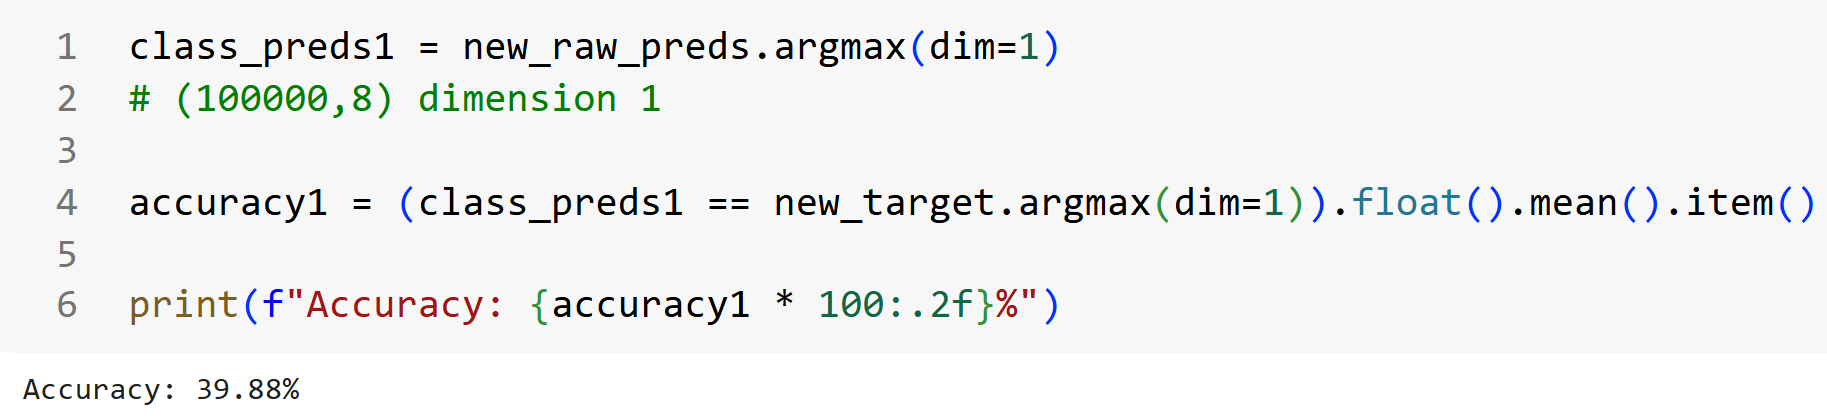
\includegraphics[width=1\linewidth]{images/trainingResultTST.png}
    \caption{Accuracy of TST Plus Model After Training it on Balanced Toyota Smarthome Untrimmed Dataset}
    \label{fig:tst accuracy}
\end{figure}
